\documentclass[a4paper]{article} 
\usepackage{graphicx} 
\usepackage[ngerman]{babel} 
\usepackage[ansinew]{inputenc} 
\usepackage[T1]{fontenc} 
\usepackage{tgpagella} 
\usepackage{geometry} 
\usepackage{color} 
\usepackage{microtype} 
\usepackage{minted}
\usepackage{caption}
\usepackage[headsepline,footsepline]{scrpage2}
\usepackage{textcomp}
\usepackage{pdfpages}
\usepackage{mdframed}



\makeatletter
\renewcommand\minted@pygmentize[2][\jobname.pyg]{
  \def\minted@cmd{pygmentize -l #2 -f latex -F tokenmerge
    \minted@opt{gobble} \minted@opt{texcl} \minted@opt{mathescape}
    \minted@opt{startinline} \minted@opt{funcnamehighlighting}
    \minted@opt{linenos} -P "verboptions=\minted@opt{extra}"
    -O encoding=UTF-8,outencoding=iso-8859-1 -o \jobname.out.pyg #1}
  \immediate\write18{\minted@cmd}
  % For debugging, uncomment:
  %\immediate\typeout{\minted@cmd}
  \ifthenelse{\equal{\minted@opt@bgcolor}{}}
   {}
   {\begin{minted@colorbg}{\minted@opt@bgcolor}}
  \input{\jobname.out.pyg}
  \ifthenelse{\equal{\minted@opt@bgcolor}{}}
   {}
   {\end{minted@colorbg}}
  \DeleteFile{\jobname.out.pyg}}
\makeatother


\title{Dokumentation - 6 Übung}
\author{Roman Lumetsberger}
\date{\today}

\newmintedfile[ccode]{cpp}{
               linenos,
               numbersep=5pt,
               frame=lines,
               framesep=2mm
}

\newmintedfile[javacode]{java}{
               linenos,
               numbersep=5pt,
               frame=lines,
               tabsize=2,
               framesep=2mm,
}
\newmintedfile[csscode]{css}{
               linenos,
               numbersep=5pt,
               frame=lines,
               tabsize=2,
               framesep=2mm,
}
\newmintedfile[sqlcode]{sql}{
               linenos,
               numbersep=5pt,
               frame=lines,
               tabsize=2,
               framesep=2mm,
}
\captionsetup{
  font=footnotesize,
  justification=raggedright,
  singlelinecheck=false
}


\newcommand{\srcDir}{../Beispiel/src/at/lumetsnet/caas/}
\newcommand{\testDir}{../Beispiel/test/at/lumetsnet/caas/test/}

\definecolor{lineColor}{RGB}{151,0,0}
\pagestyle{scrheadings}
\clearscrheadfoot
\begin{document}
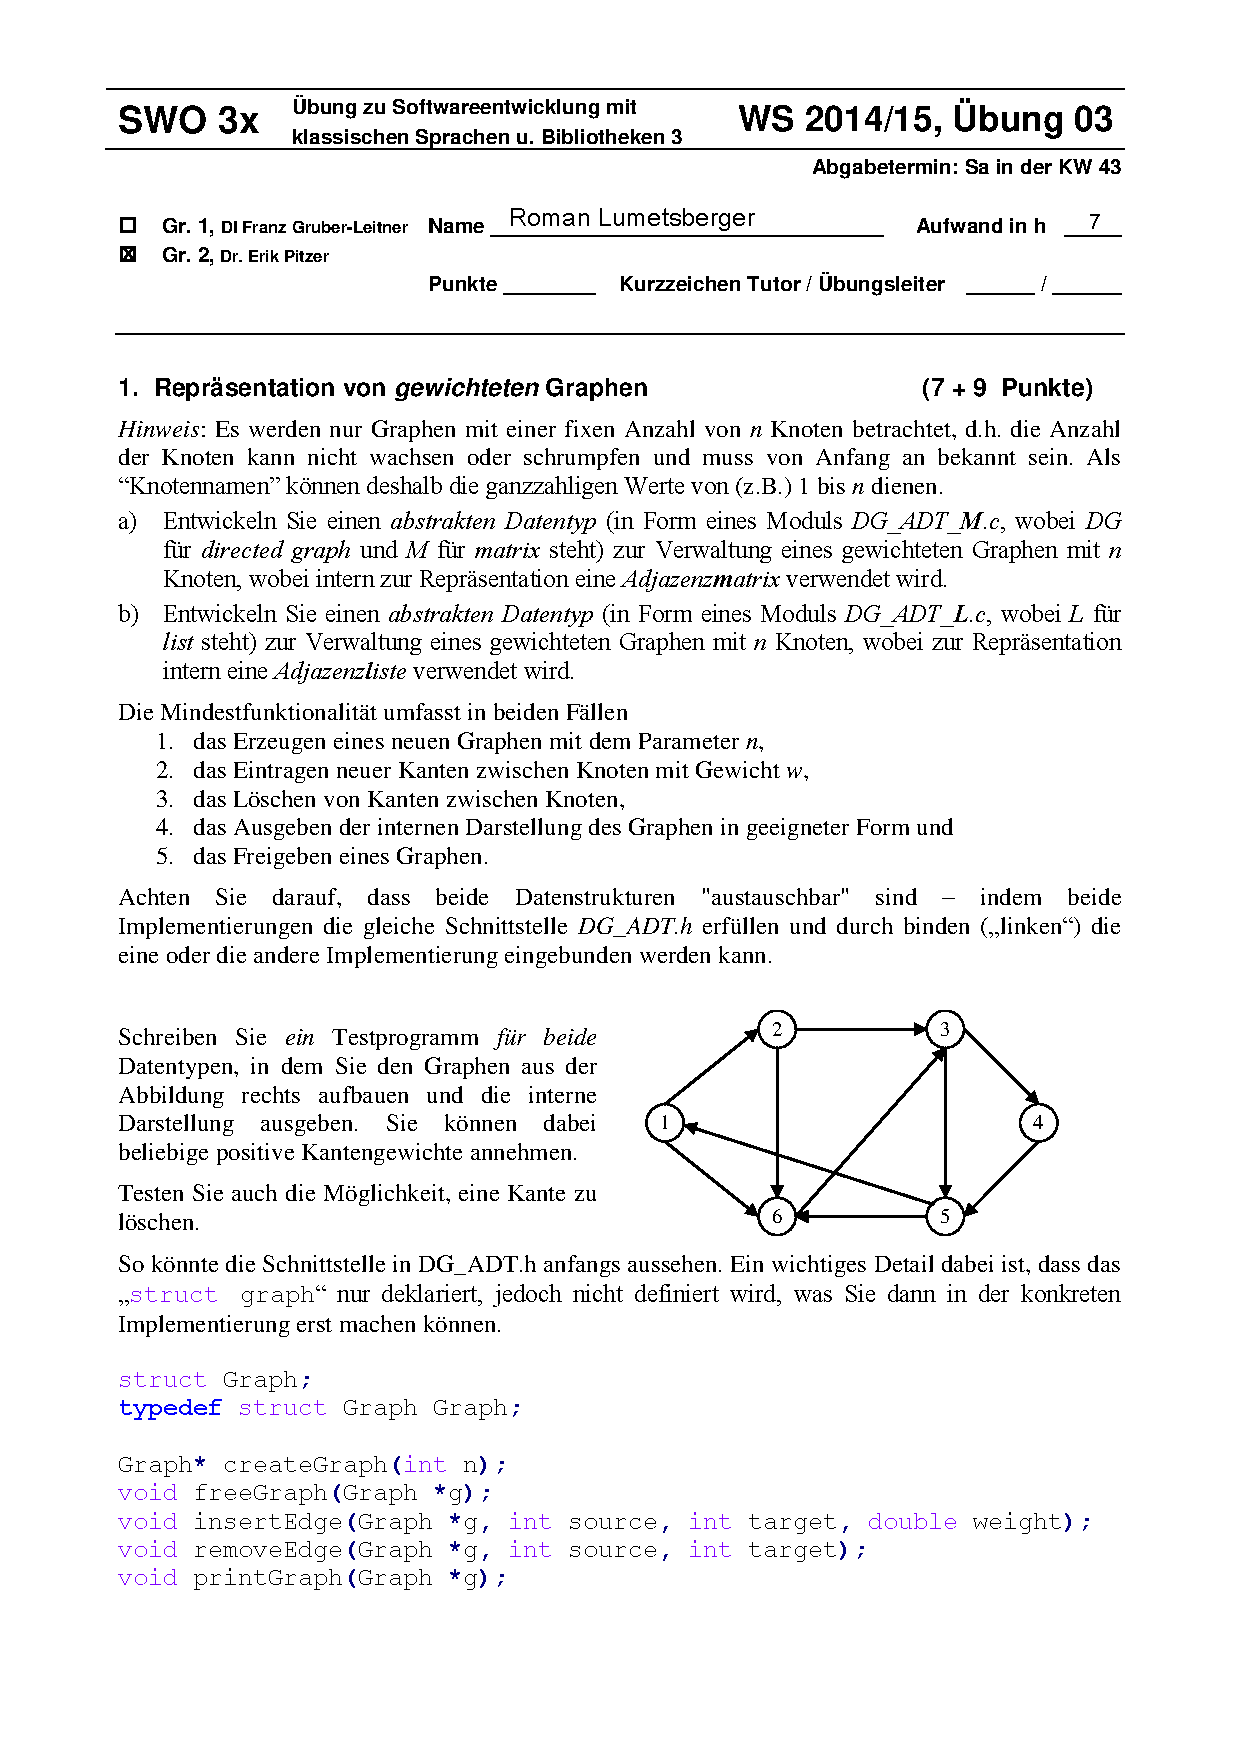
\includepdf[pages=-]{angabe.pdf}

\ihead{SWO3 WS 2014/15 - �bung 03}
\ifoot{Roman Lumetsberger}
\cfoot{1310307026}
\ofoot{Seite \pagemark}

\section{Aufgabe 1 - Repr�sentation von gewichteten Graphen}
\subsection{L�sungsidee}
Zu Beginn muss das Interface \textit{dg\_adt.h} definiert werden. Dabei wird die Schnittstelle der Angabe verwendet.
Wichtig ist hier, dass der Type \textit{graph} deklariert wird, ohne eine konkrete interne Struktur vorzugeben.\newline
\textbf{In diesem Beispiel werden als Knotennamen 1 - n verwendet, wobei intern die Speicherung mit Index 0 erfolgt.}
\subsubsection{Adjazenzmatrix}
Beim diesem Beispiel wird der Graph als Adjazenzmatrix implementiert. \newline
Eine Adjazenzmatrix ist eine Matrix mit n * n Elementen. Dabei wird f�r jede m�gliche Kombination das Gewicht der Kante gespeichert. \newline
Ist das Gewicht Null, dann existiert keine Kante zwischen den Knoten.
\begin{itemize}
\item Beim Einf�gen einer Kante wird einfach das Gewicht an die richtige Stelle der Matrix geschrieben.
\item Beim L�schen wird der Wert wieder auf Null gesetzt.
\end{itemize} 
\textbf{Speicherverwaltung}\newline
Beim Erstellen des Graphen wird die gesamte Matrix allokiert, beim L�schen wird sie wieder freigegeben.

\subsubsection{Adjazenzliste}
Bei dieser Variante der Speicherung eines Graphen wird ein Array verwendet, welches f�r jeden Knoten eine Liste der Kanten bereitstellt. \newline
Die Implementierung verwendet eine einfach verkette Liste.

\begin{itemize}
\item Beim Einf�gen einer Kante wird ein neues Element in die Liste des Ausgangsknoten eingef�gt
\item Beim L�schen wird das Element der Liste wieder entfernt
\end{itemize}
\textbf{Speicherverwaltung}\newline
Beim Erstellen des Graphen wird nur das Array mit den Zeigern auf die Liste allokiert.  
\begin{itemize}
\item Wird ein Element eingef�gt, wird ein neues Listenelement allokiert und in die Liste eingef�gt.
\item Beim L�schen einer Kante muss das Element gesucht, die Verkettung der Liste aktualisiert und das Element freigegeben werden.
\item Beim L�schen des Graphen m�ssen zuerst die Listenelemente, dann das Array der Knoten und dann der Graph selbst freigegeben werden.
\end{itemize}


\pagebreak
\subsection{Sourcecode}
\subsubsection{Makefile}
In der Abgabe Zip Datei ist ein Makefile enthalten, dass f�r jede Implementierung ein Target enth�lt.
\begin{itemize}
\item Target graphm: Erstellt das Programm \textbf{graphm}, das als Implementierung die Adjazenzmatrix (dg\_adt\_m.o) verwendet
\item Target graphl: Erstellt das Programm \textbf{graphl}, das als Implementierung die Adjazenzliste (dg\_adt\_l.o) verwendet
\end{itemize}
\ccode{../beispiel1/dg_adt.h}
\ccode{../beispiel1/dg_adt_m.c}
\ccode{../beispiel1/dg_adt_l.c}
\ccode{../beispiel1/graph.c}
\subsection{Testf�lle}


\subsubsection{Testfall 1 - Adjazenzmatrix}
\begin{itemize}
\item Erzeugen eines Graphen mit 6 Knoten
\item Ausgeben des leeren Graphen
\item Hinzuf�gen aller Kanten des Angabenbeispiels
\item �berschreiben einer Kante mit einem anderen Gewicht
\item Ausgeben des Graphen
\item L�schen einiger Kanten
\item Ausgeben des Graphen
\item Freigeben des Graphen
\end{itemize}
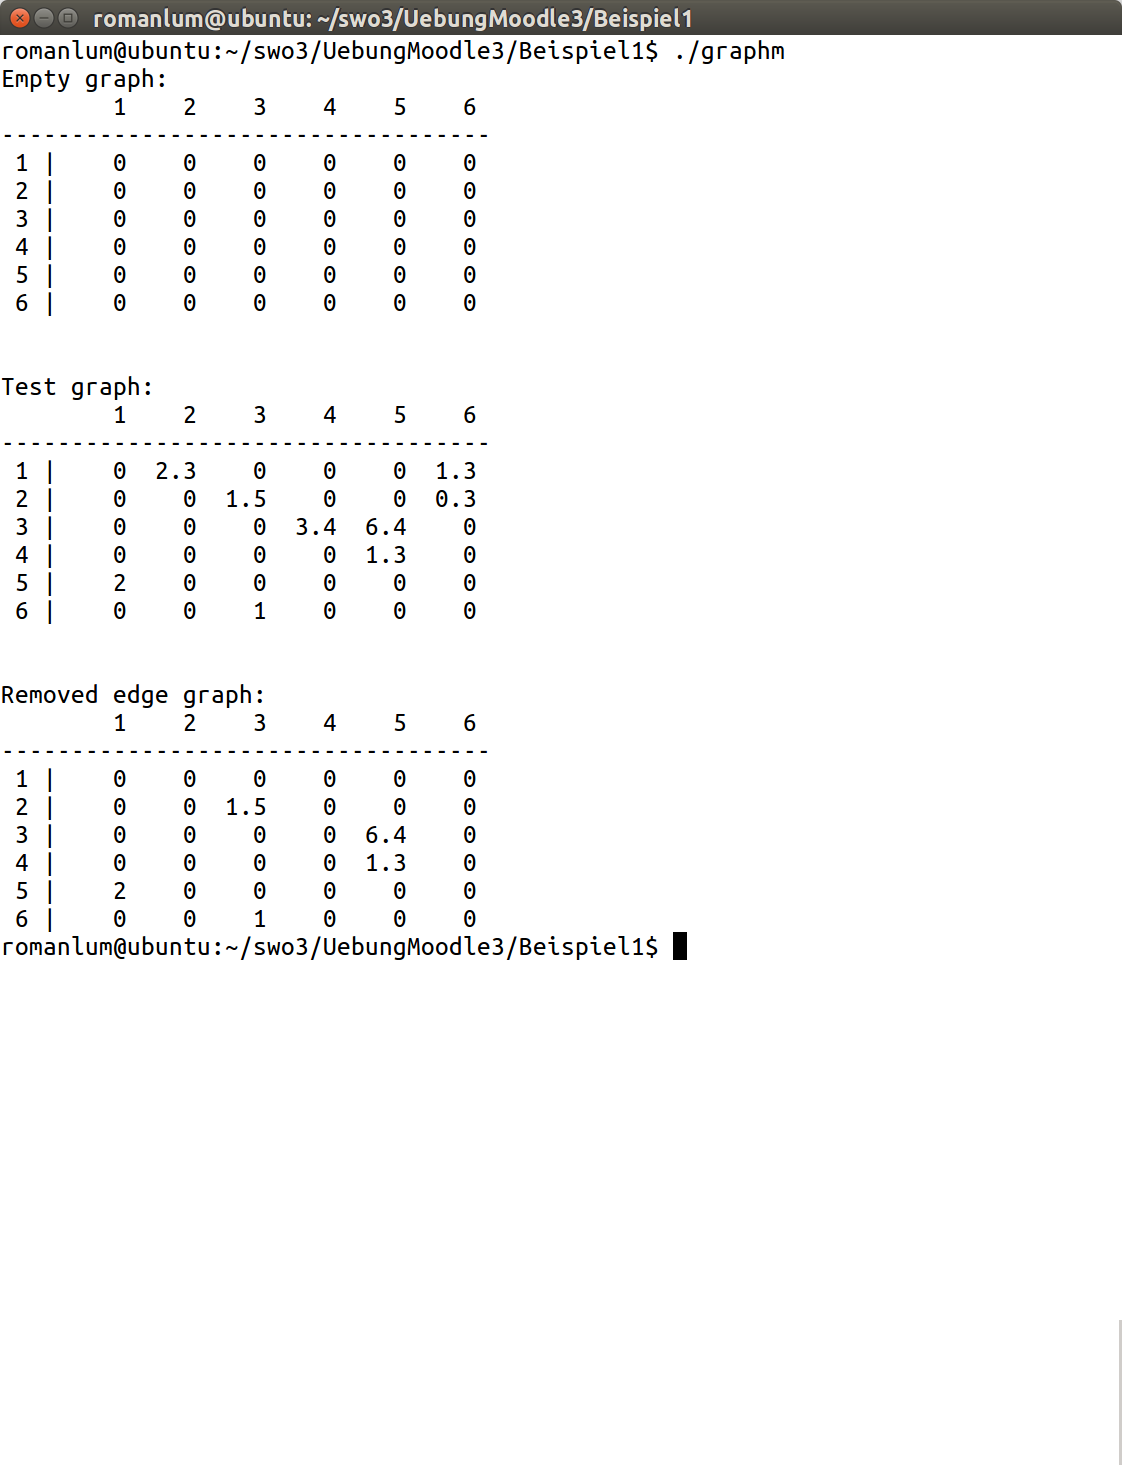
\includegraphics[width=300px, clip=true,trim=0px 000px 0px 0px]{../screenshots/beispiel1/1.png}

\subsubsection{Testfall 2 - Adjazenzmatrix - Valgrind}
Gleiche Operationen wie in Testfall 1, nur diesmal mit valgrind (Memory Leak Detector) ausgef�hrt, um zu zeigen, dass der Speicher wieder korrekt freigeben wird. \newline
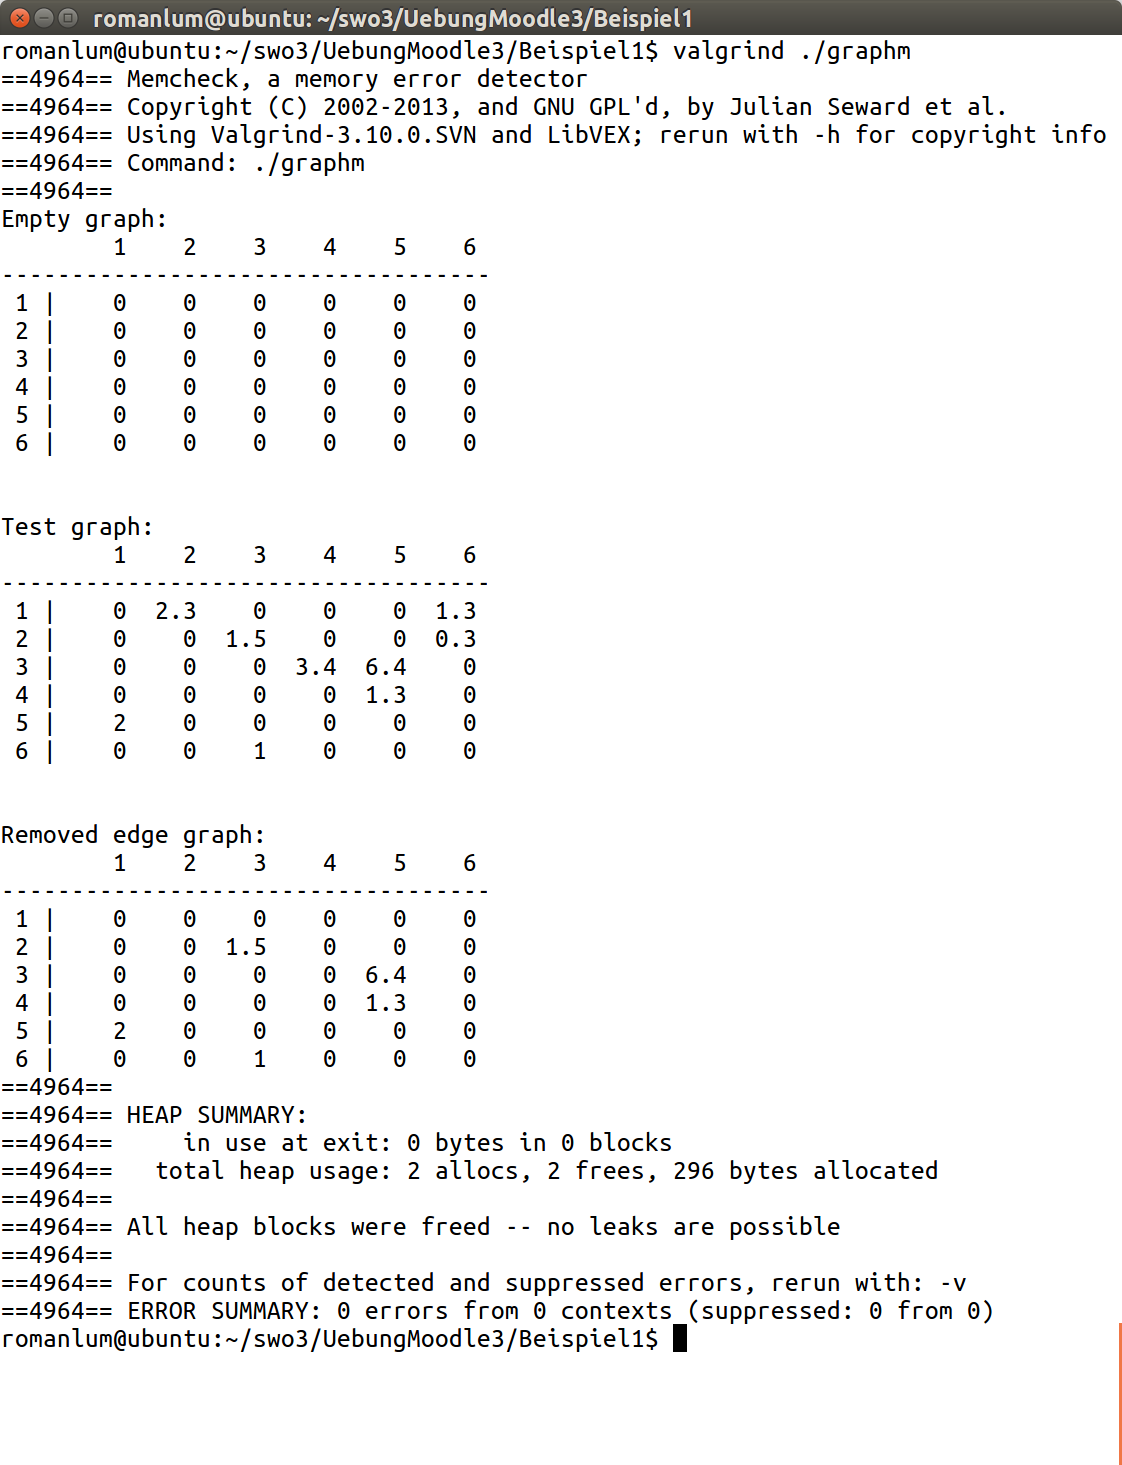
\includegraphics[width=300px, clip=true,trim=0px 000px 0px 0px]{../screenshots/beispiel1/2.png}

\subsubsection{Testfall 3 - Adjazenzliste}
Gleiche Operationen wie in Testfall 1, nur diesmal mit der Listenimplementierung\newline
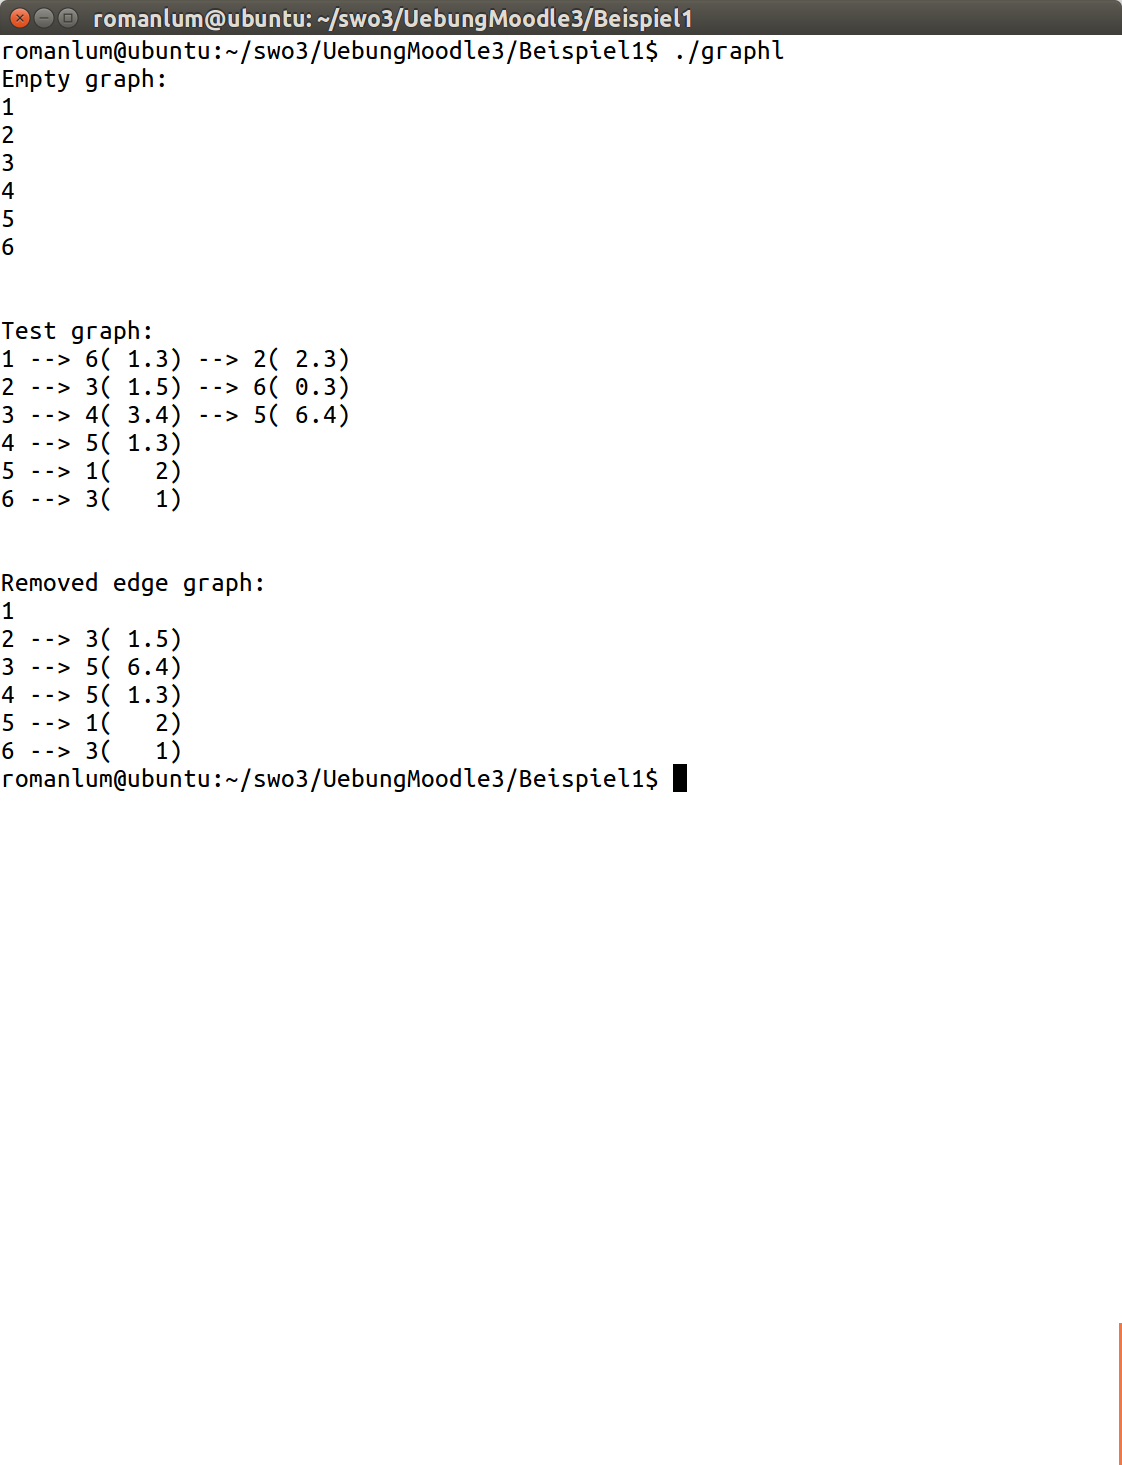
\includegraphics[width=300px, clip=true,trim=0px 000px 0px 0px]{../screenshots/beispiel1/3.png}

\subsubsection{Testfall 4 - Adjazenzliste - Valgrind}
Gleiche Operationen wie in Testfall 3, nur diesmal mit valgrind (Memory Leak Detector) ausgef�hrt, um zu zeigen, dass der Speicher wieder korrekt freigeben wird. \newline

\includegraphics[width=300px, clip=true,trim=0px 000px 0px 0px]{../screenshots/beispiel1/4.png}

\section{Aufgabe 2 - Graphenalgorithmen}
\subsection{L�sungsidee}
Um die ben�tigten Algorithmen umzusetzen werden 2 neue Methoden ben�tigt
\begin{minted}[frame=lines,
               framesep=2mm]{c}
/* gets the count of vertices */
int getVerticesCount(Graph *g);

/* gets the weight of the edge between source and target
returns 0 if there is no edge
source and target are starting with 1 */
double getEdgeWeight(Graph *g, int source, int target); 
\end{minted}
Mit diesen Methoden k�nnen dann in einer Schleife alle Knoten durchlaufen und die Kanten gepr�ft werden.

\subsubsection{invert}
Um den Graphen zu invertieren, muss zuerst ein neuer Graph mit der korrekten Anzahl an Knoten angelegt werden.\newline
Dann m�ssen alle Knoten in einer verschachtelten Schleife durchlaufen werden
\begin{itemize}
\item Gibt es eine Kante muss in den neuen Graph eine Kante in umgekehrter Richtung eingef�gt werden.
\end{itemize}
\subsubsection{isReflexive}
Ein Graph ist reflexiv, wenn jeder Knoten eine Kante auf sich selbst hat.\newline
D.h. alle Knoten durchlaufen und pr�fen, ob eine Kante zu sich selbst existiert.

\subsubsection{isSymmetric}
Ein Graph ist symmetrisch, wenn jede Kante in beiden Richtungen vorhanden ist.\newline
D.h. alle Kanten durchlaufen und pr�fen, ob auch die Kante in umgekehrter Richtung existiert.

\subsubsection{isAsymmetric}
Ein Graph ist asymmetrisch, wenn jede Kante nur in einer Richtungen vorhanden ist.\newline
D.h. alle Kanten durchlaufen und pr�fen, dass keine Kante in umgekehrter Richtung existiert.


\subsubsection{isTransitivev}
Ein Graph ist transitiv, wenn jeder Knoten, der �ber einen anderen Knoten erreichbar ist, auch eine direkte Kante hat.\newline
D.h. alle Knoten und deren Pfade durchlaufen und pr�fen ob auch eine direkte Verbindung vom Ausgangsknoten existiert.

\subsubsection{printGraphProperties}
Wendet die oben angef�hrten Funktionen auf den Graph an und gibt die Ergebnisse aus.
	
\subsection{Sourcecode}
\subsubsection{Makefile}
In der Abgabe Zip Datei ist ein Makefile enthalten, dass f�r jede Implementierung ein Target enth�lt.
\begin{itemize}
\item Target graphm: Erstellt das Programm \textbf{graphm}, das als Implementierung die Adjazenzmatrix (dg\_adt\_m.o) verwendet
\item Target graphl: Erstellt das Programm \textbf{graphl}, das als Implementierung die Adjazenzliste (dg\_adt\_l.o) verwendet
\end{itemize}
\ccode{../beispiel2/dg_adt.h}
\ccode{../beispiel2/dg_adt_m.c}
\ccode{../beispiel2/dg_adt_l.c}
\ccode{../beispiel2/graph_algs.h}
\ccode{../beispiel2/graph_algs.c}
\ccode{../beispiel2/graph.c}
\subsection{Testf�lle}

\subsubsection{Testfall 1 - invers}
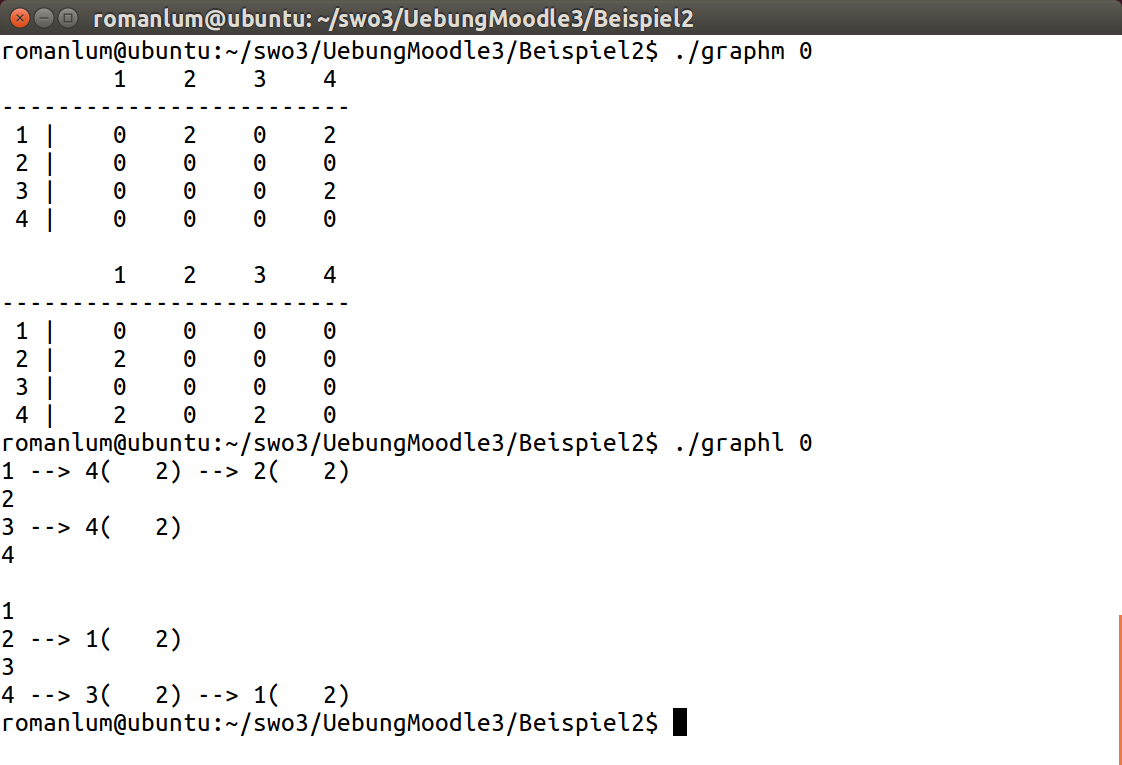
\includegraphics[width=300px, clip=true,trim=0px 000px 0px 0px]{../screenshots/beispiel2/0.png}

\subsubsection{Testfall 2 - reflexiv}
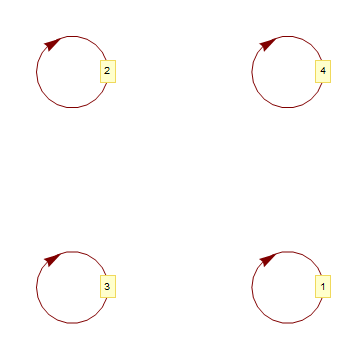
\includegraphics[width=200px, clip=true,trim=0px 000px 0px 0px]{./graphen/1.png}\newline
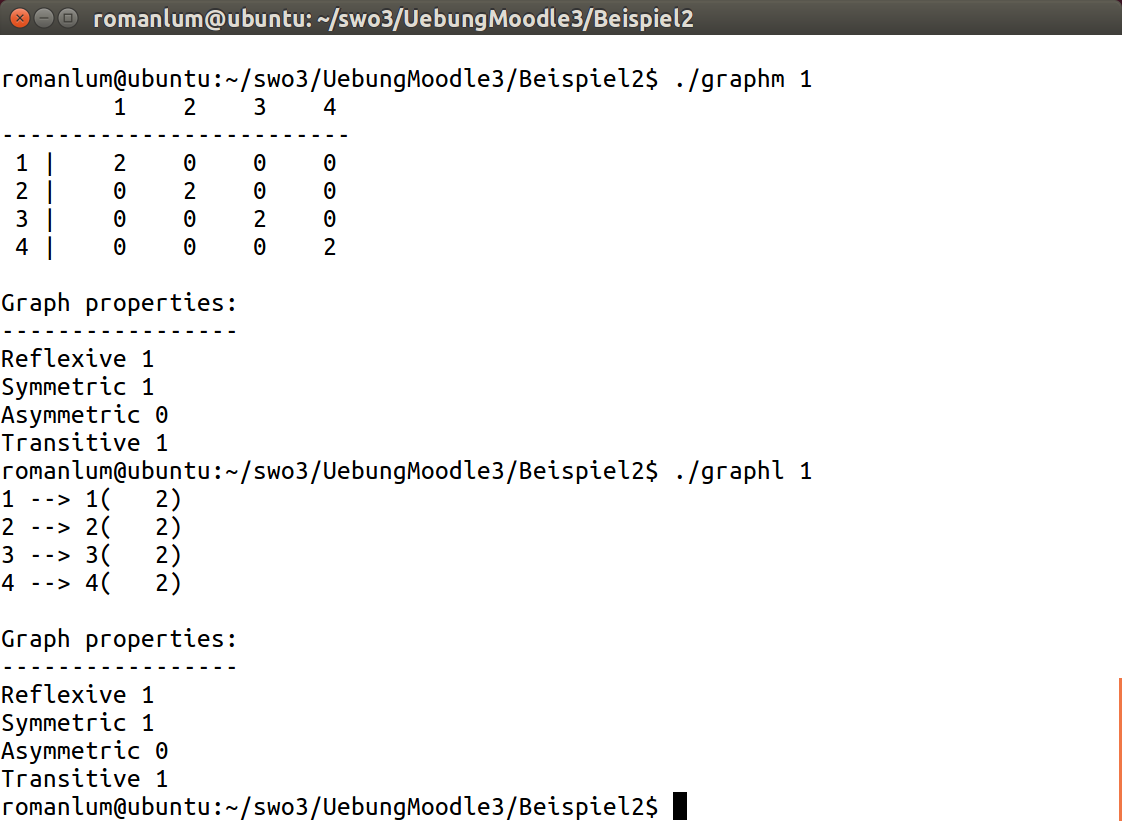
\includegraphics[width=300px, clip=true,trim=0px 000px 0px 0px]{../screenshots/beispiel2/1.png}

\subsubsection{Testfall 3 - symmetrisch}

\includegraphics[width=200px, clip=true,trim=0px 000px 0px 0px]{./graphen/2.png}\newline
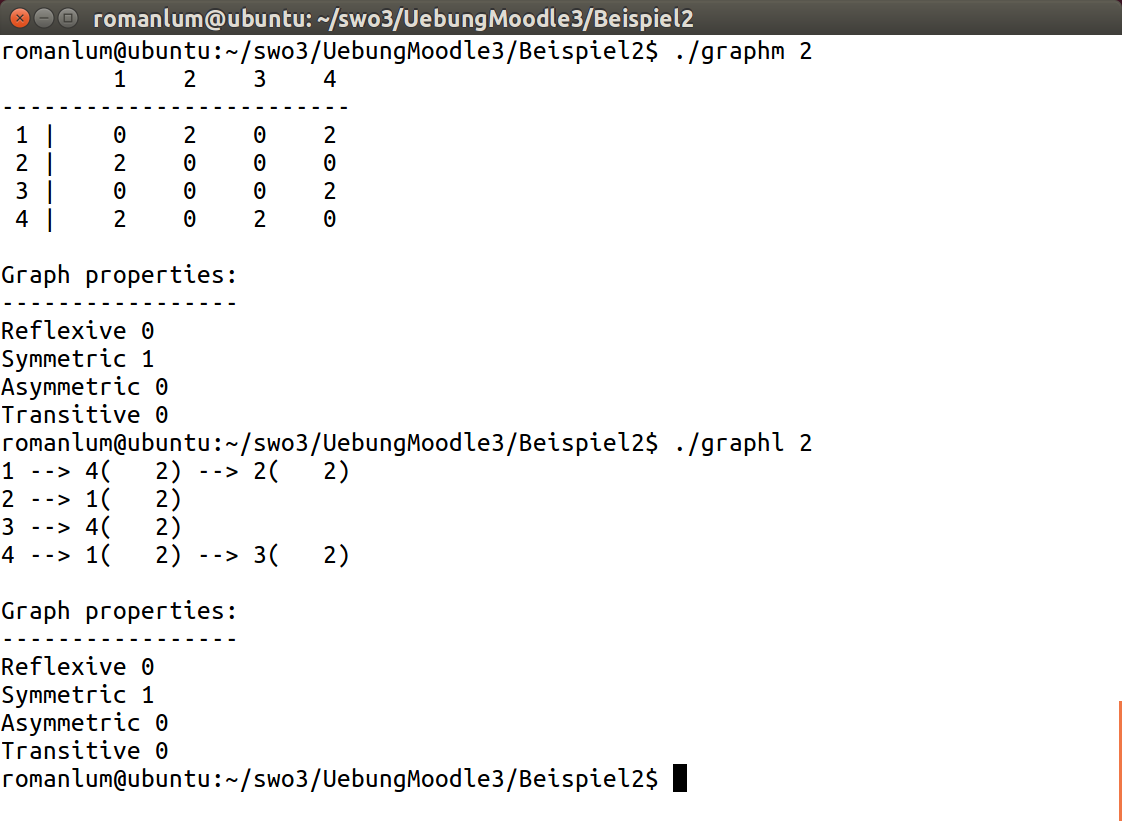
\includegraphics[width=300px, clip=true,trim=0px 000px 0px 0px]{../screenshots/beispiel2/2.png}

\subsubsection{Testfall 4 - asymmetrisch}

\includegraphics[width=200px, clip=true,trim=0px 000px 0px 0px]{./graphen/3.png}\newline
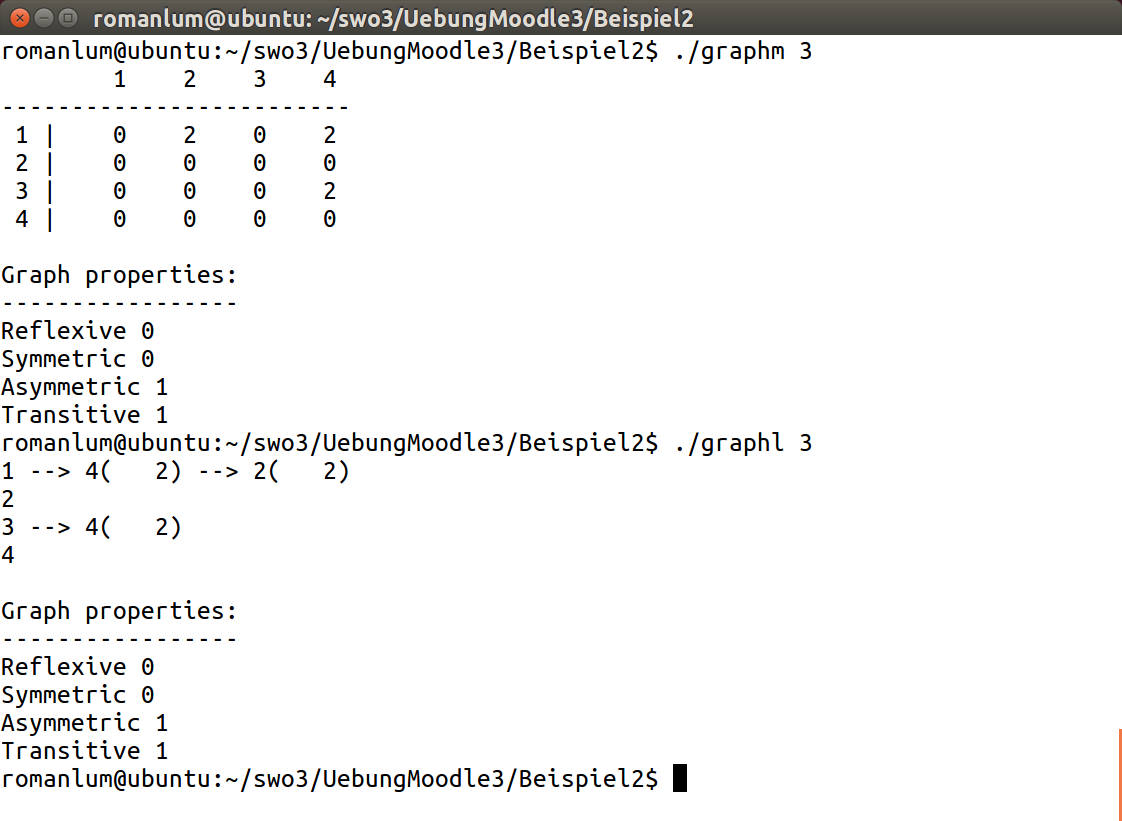
\includegraphics[width=300px, clip=true,trim=0px 000px 0px 0px]{../screenshots/beispiel2/3.png}

\subsubsection{Testfall 5 - transitiv}

\includegraphics[width=200px, clip=true,trim=0px 000px 0px 0px]{./graphen/4.png}\newline

\includegraphics[width=300px, clip=true,trim=0px 000px 0px 0px]{../screenshots/beispiel2/4.png}

\subsubsection{Testfall 6 - reflexiv, symmetrisch, transitiv}
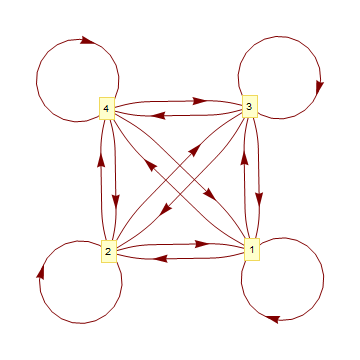
\includegraphics[width=200px, clip=true,trim=0px 000px 0px 0px]{./graphen/5.png}\newline
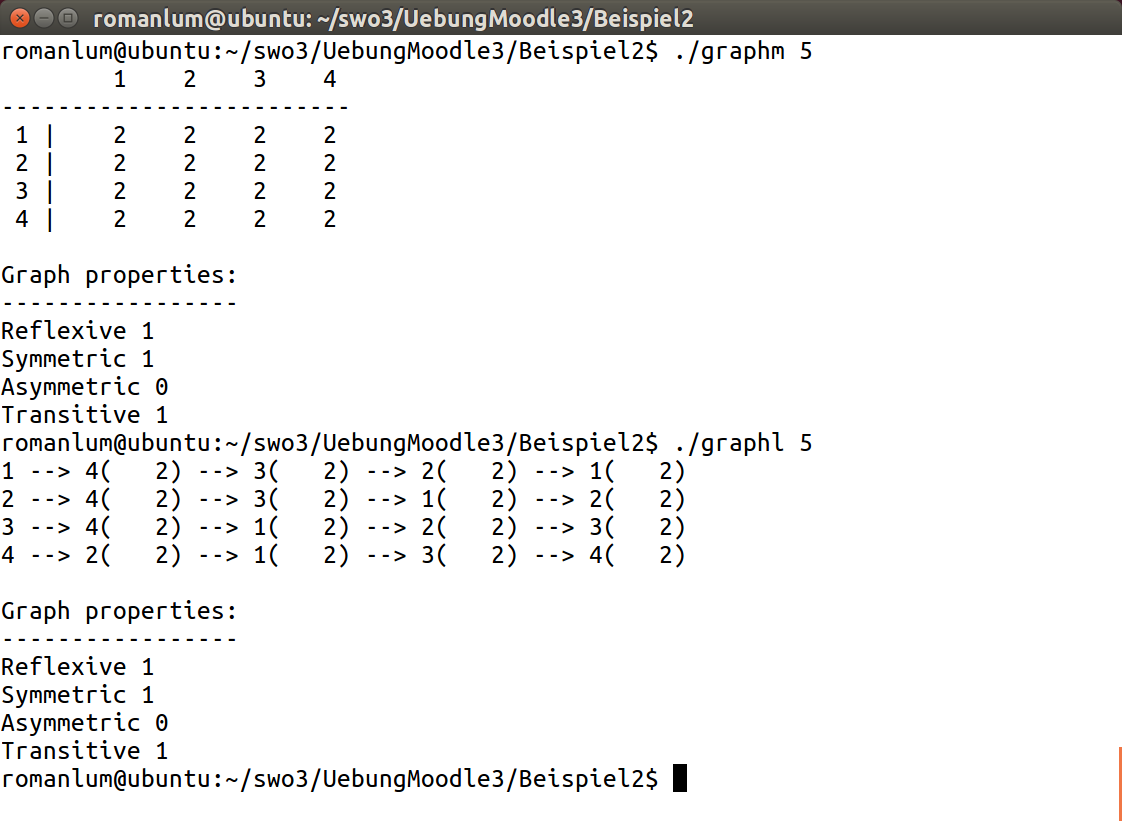
\includegraphics[width=300px, clip=true,trim=0px 000px 0px 0px]{../screenshots/beispiel2/5.png}

\end{document}